\chapter{Durchführung des Passiv Radar}
\section{Einführung}
\section{Messung}
\subsection{Messpunkt}
Der Messpunkt ist so gewählt das sowohl der Stuttgarter Flughaffen als auch der Stuttgarter Fernsehturm für das Radar sichtbar sind und außerdem gut vom Studentenwohnheim Geschwister-Scholl-Str. gut erreichbar war. Das Passivradar wurde in der Nähe des Segelflughafen Esslingen aufgebaut, die genaue Position können ist in Abbildung /ref{Maps} auf Google Maps erkennen.

\begin{figure}
    \centering
    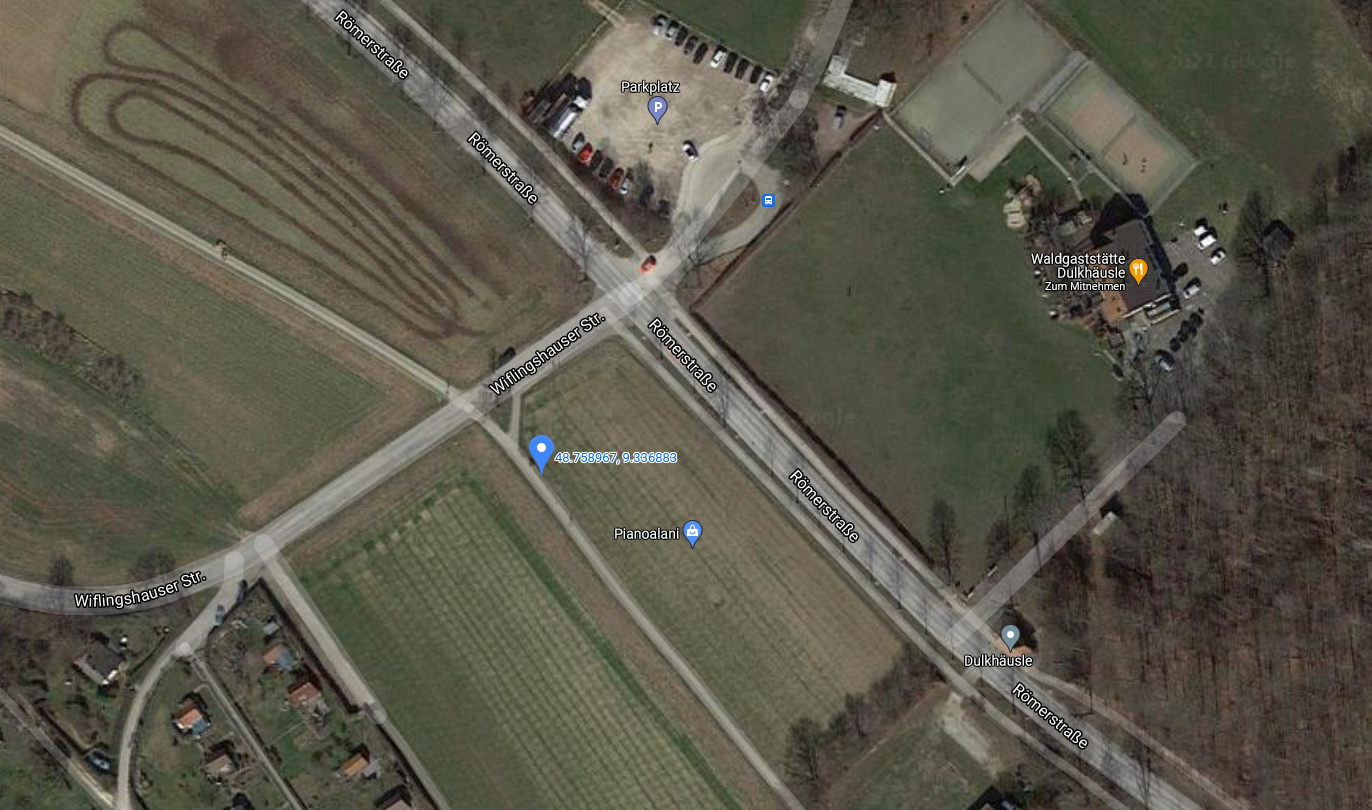
\includegraphics[width=\textwidth]{images/Maps_Messpunkt.png}
    \caption{Possition des Messpunkt}\label{Maps}
\end{figure}

\subsection{Messaufbau}

\begin{figure}
    \centering
    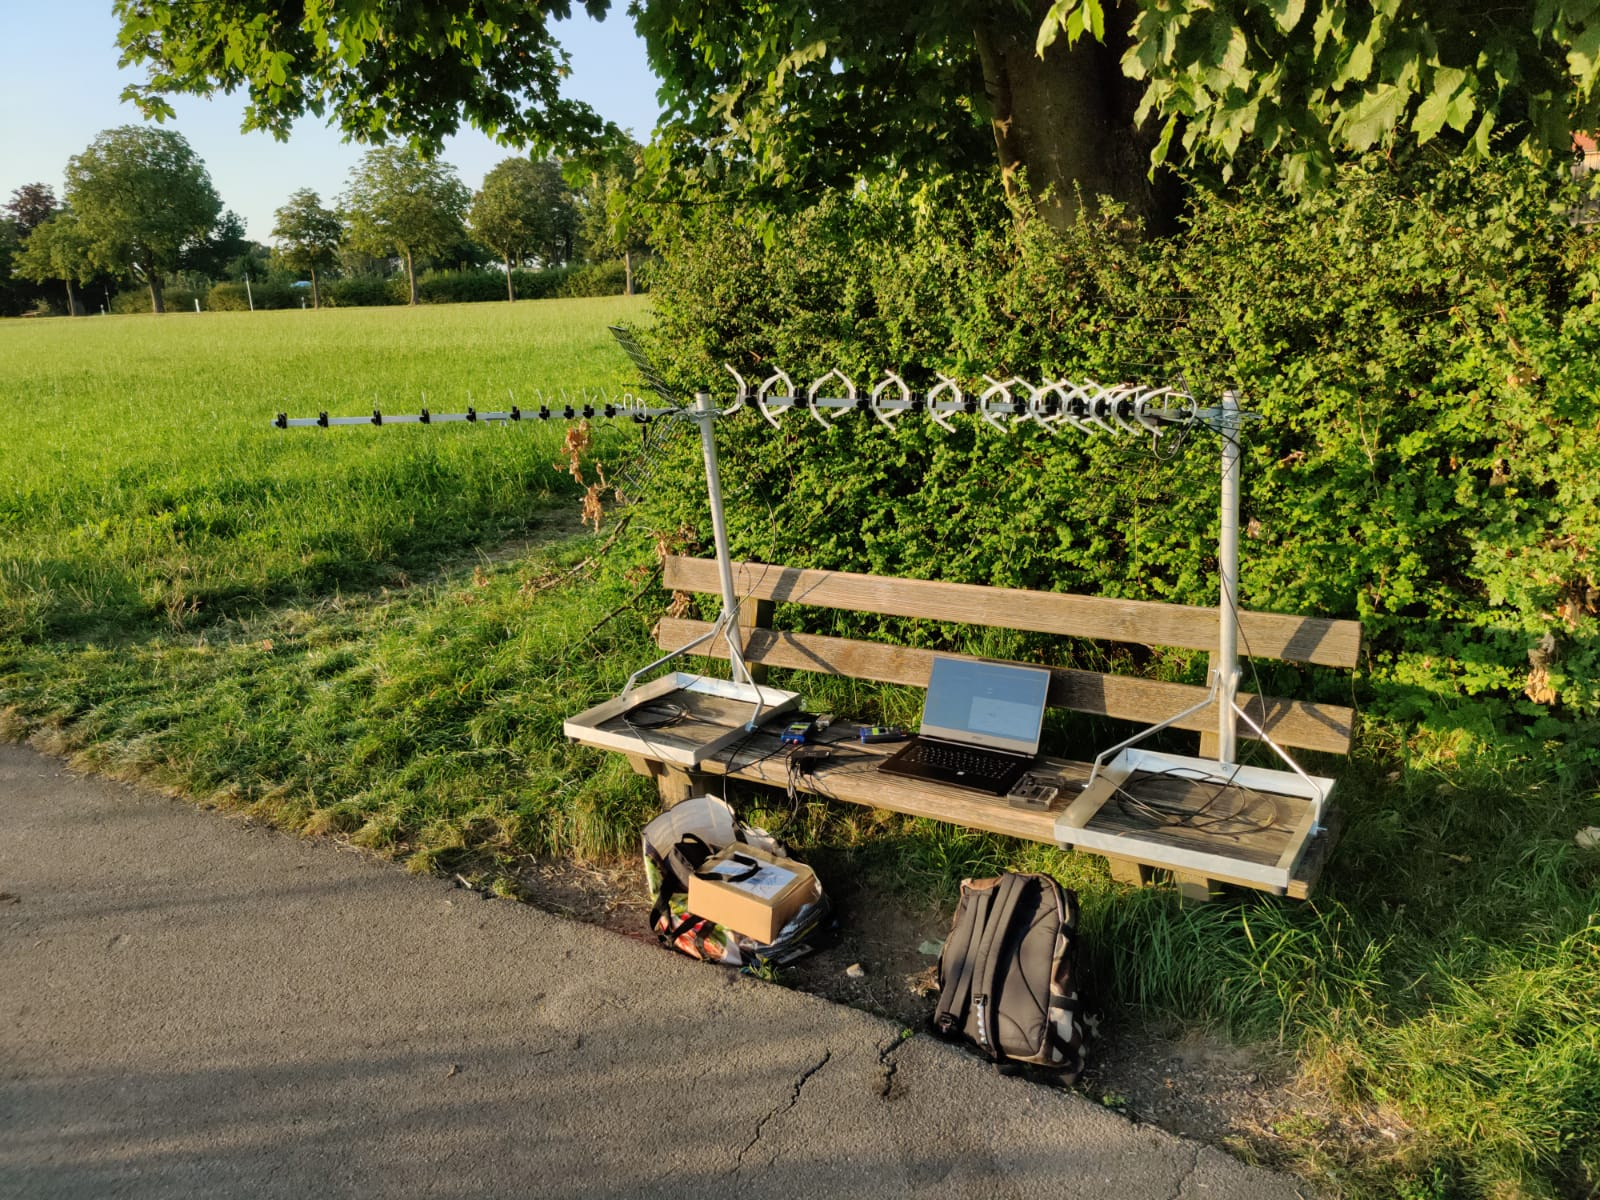
\includegraphics[width=\textwidth]{images/Messaufbau.jpg}
    \caption{Aufbau der Messung}\label{Messaufbau}
\end{figure}
